\documentclass[11pt]{article}

\usepackage[utf8]{inputenc}
\usepackage[T1]{fontenc}
\usepackage[brazilian]{babel}
\usepackage[a4paper,margin=2.5cm]{geometry}
\usepackage{graphicx}
\usepackage{booktabs}
\usepackage{longtable}
\usepackage{caption}
\usepackage{float}
\usepackage{hyperref}

\title{Segmentação Automática de B-Lines em Ultrassom Pulmonar: \\
Comparação de Arquiteturas e Representações de Saída}
\author{}
\date{Outubro de 2026}

\begin{document}

\maketitle

% ============================================================
\section{Contexto e Objetivo}
% ============================================================

O projeto estuda a segmentação automática de B-Lines em ultrassom pulmonar. A ideia
central não é apenas treinar um modelo, mas montar uma estrutura de experimentos que
permita comparar arquiteturas diferentes usando o mesmo dataset e split, registrando
as diferenças de protocolo e aplicando métricas COCO comuns sempre que possível. A
pergunta central é como a representação e a supervisão geométrica afetam a
localização de B-Lines com poucas anotações.

As anotações originais estão no formato YOLO Polygon: cada B-Line é um quadrilátero
de 4 vértices (classe $x_1\ y_1\ x_2\ y_2\ x_3\ y_3\ x_4\ y_4$, coordenadas
normalizadas).

% ============================================================
\section{Dataset}
% ============================================================

O conjunto de treino tem 256 imagens. O conjunto de validação tem 75 imagens e 115
instâncias anotadas (1,53 B-Lines por imagem, em média). Existe ainda um conjunto de
teste com 70 imagens, mas sem rótulo até o momento.

Como o teste não tem anotação, todos os números reportados neste trabalho vêm do
conjunto de validação --- o mesmo usado para acompanhar o treino. Isso é discutido
na Seção~\ref{sec:limitacoes} como limitação.

A validação contém 75 arquivos de rótulo válidos e 115 instâncias, sem imagens
negativas. Na auditoria do treino, duas instâncias tinham cinco vértices, apesar de
o formato esperado ser um quadrilátero. Para tornar os loaders consistentes, ambas
foram convertidas para quatro vértices removendo o ponto cuja exclusão minimiza a
área do triângulo local. A correção e as linhas originais estão registradas em
\texttt{docs/annotation\_corrections.json}; essa aproximação altera uma das áreas
em 7,7\% e não confirma a intenção do anotador.

% ============================================================
\section{Protocolo Experimental}
% ============================================================

Mask R-CNN, Faster R-CNN e Polygon Head usam Detectron2, backbone ResNet-50 com FPN,
pesos pré-treinados no COCO, batch de 4 imagens, taxa de aprendizado de 0,00025 e
2.000 iterações. A cada 100 iterações há avaliação e checkpoint. A seleção é
alinhada à tarefa: segm/AP para Mask R-CNN, bbox/AP para Faster R-CNN e
segm\_polygon/AP para Polygon Head. Um hook adicional calcula a loss de validação
sem augmentations aleatórias.

Os baselines e as quatro novas configurações poligonais foram executados com três
seeds (0, 1 e 2). Os resultados atuais são apresentados como média e desvio-padrão
amostral entre seeds. As diferenças entre framework, augmentations e hiperparâmetros
do YOLO permanecem como fatores de confusão na comparação entre famílias de modelos.

O YOLOv11n usa o framework Ultralytics e seu protocolo de treino (31 épocas), sobre
os mesmos splits. Suas predições são convertidas para COCO e avaliadas com COCOeval,
em vez de comparar a métrica nativa do Ultralytics com as dos demais modelos.

% ============================================================
\section{Mask R-CNN (baseline)}
\label{sec:maskrcnn}
% ============================================================

Arquitetura de referência do projeto: detecta a caixa delimitadora do objeto e
prevê uma máscara binária livre, pixel a pixel, para cada instância.

Uma execução exploratória anterior mostrou sinais de overfitting: a loss de treino
cai continuamente até aproximadamente 0,28, mas a loss de validação para de melhorar
por volta da iteração 900--1400 (mínimo de 0,44) e volta a subir, chegando a 0,51 na
iteração final (Figura~\ref{fig:mask_loss}). Nessa mesma execução, o checkpoint
final não era o melhor: o AP de segmentação atingiu seu pico na iteração 1399
(40,61) e caiu para 38,33 na iteração 2000 (Figura~\ref{fig:mask_ap}). Por isso
passou-se a selecionar o melhor checkpoint em vez de sempre usar o último --- essa
mudança sozinha elevou o
AP de segmentação reportado de 36,7 para 40,6. Esses valores descrevem uma execução
anterior e não a média das três seeds da rodada atual, cujos resultados são
apresentados na tabela consolidada da Seção~\ref{sec:resumo}.

\begin{table}[H]
\centering
\caption{Mask R-CNN na rodada atual: média $\pm$ desvio-padrão amostral de três
seeds. A análise de loss e iteração descrita acima pertence à execução exploratória
anterior.}
\begin{tabular}{lccc}
\toprule
Saída & AP & AP50 & AP75 \\
\midrule
Caixa delimitadora (bbox) & $56,12\pm1,74$ & $91,23\pm2,01$ & $59,89\pm4,13$ \\
Segmentação (segm) & $42,88\pm0,70$ & $86,14\pm0,98$ & $35,98\pm1,09$ \\
\bottomrule
\end{tabular}
\end{table}

Na rodada atual, a avaliação por instância de máscara, com matching um-para-um e
IoU $\geq0{,}50$, obteve precisão de $79,01\pm5,83\%$, recall de
$88,99\pm4,79\%$ e F1 de $83,47\pm1,15\%$. O limiar que maximiza F1 na validação
foi $0,67\pm0,10$. A execução exploratória anterior reportou outros valores de
IoU/Dice e threshold; eles não são agregados comparáveis à métrica da rodada atual.
Naquela análise anterior, foram registrados IoU médio 0,52 (mediana 0,65), Dice
médio 0,61 (mediana 0,78), precisão 0,59, recall 0,67 e confiança média 0,91. No
threshold anterior de 0,875, o F1 reportado foi 0,82 (precisão 0,81, recall 0,83).

Vale registrar que, ao inspecionar as máscaras visualmente com o threshold padrão
(0,50), apareciam máscaras borradas e detecções extras (2,31 por imagem, contra
1,53 reais). Usando o threshold ótimo do próprio modelo, esse problema quase
desapareceu --- parte do que parecia ``modelo ruim'' era, na verdade, visualização
calibrada de forma inadequada.

\begin{figure}[H]
\centering
\includegraphics[width=0.8\linewidth]{figures/mask_rcnn/train_vs_val_loss.png}
\caption{Loss de treino vs.\ validação ao longo das 2000 iterações. A validação
para de melhorar por volta da iteração 1000 e volta a subir no final.}
\label{fig:mask_loss}
\end{figure}

\begin{figure}[H]
\centering
\includegraphics[width=0.8\linewidth]{figures/mask_rcnn/val_segm_ap.png}
\caption{AP de segmentação de validação ao longo do treino. O pico ocorre antes da
iteração final.}
\label{fig:mask_ap}
\end{figure}

\begin{figure}[H]
\centering
\includegraphics[width=0.8\linewidth]{figures/mask_rcnn/coco_pr_curves.png}
\caption{Curva Precisão--Recall oficial (COCOeval) para a tarefa de segmentação.}
\label{fig:mask_pr}
\end{figure}

\begin{figure}[H]
\centering
\includegraphics[width=0.6\linewidth]{figures/predictions/mask_rcnn_1646467410642.png}
\caption{Exemplo de predição (verde: anotação real; vermelho: máscara prevista).}
\label{fig:mask_pred}
\end{figure}

\begin{figure}[H]
\centering
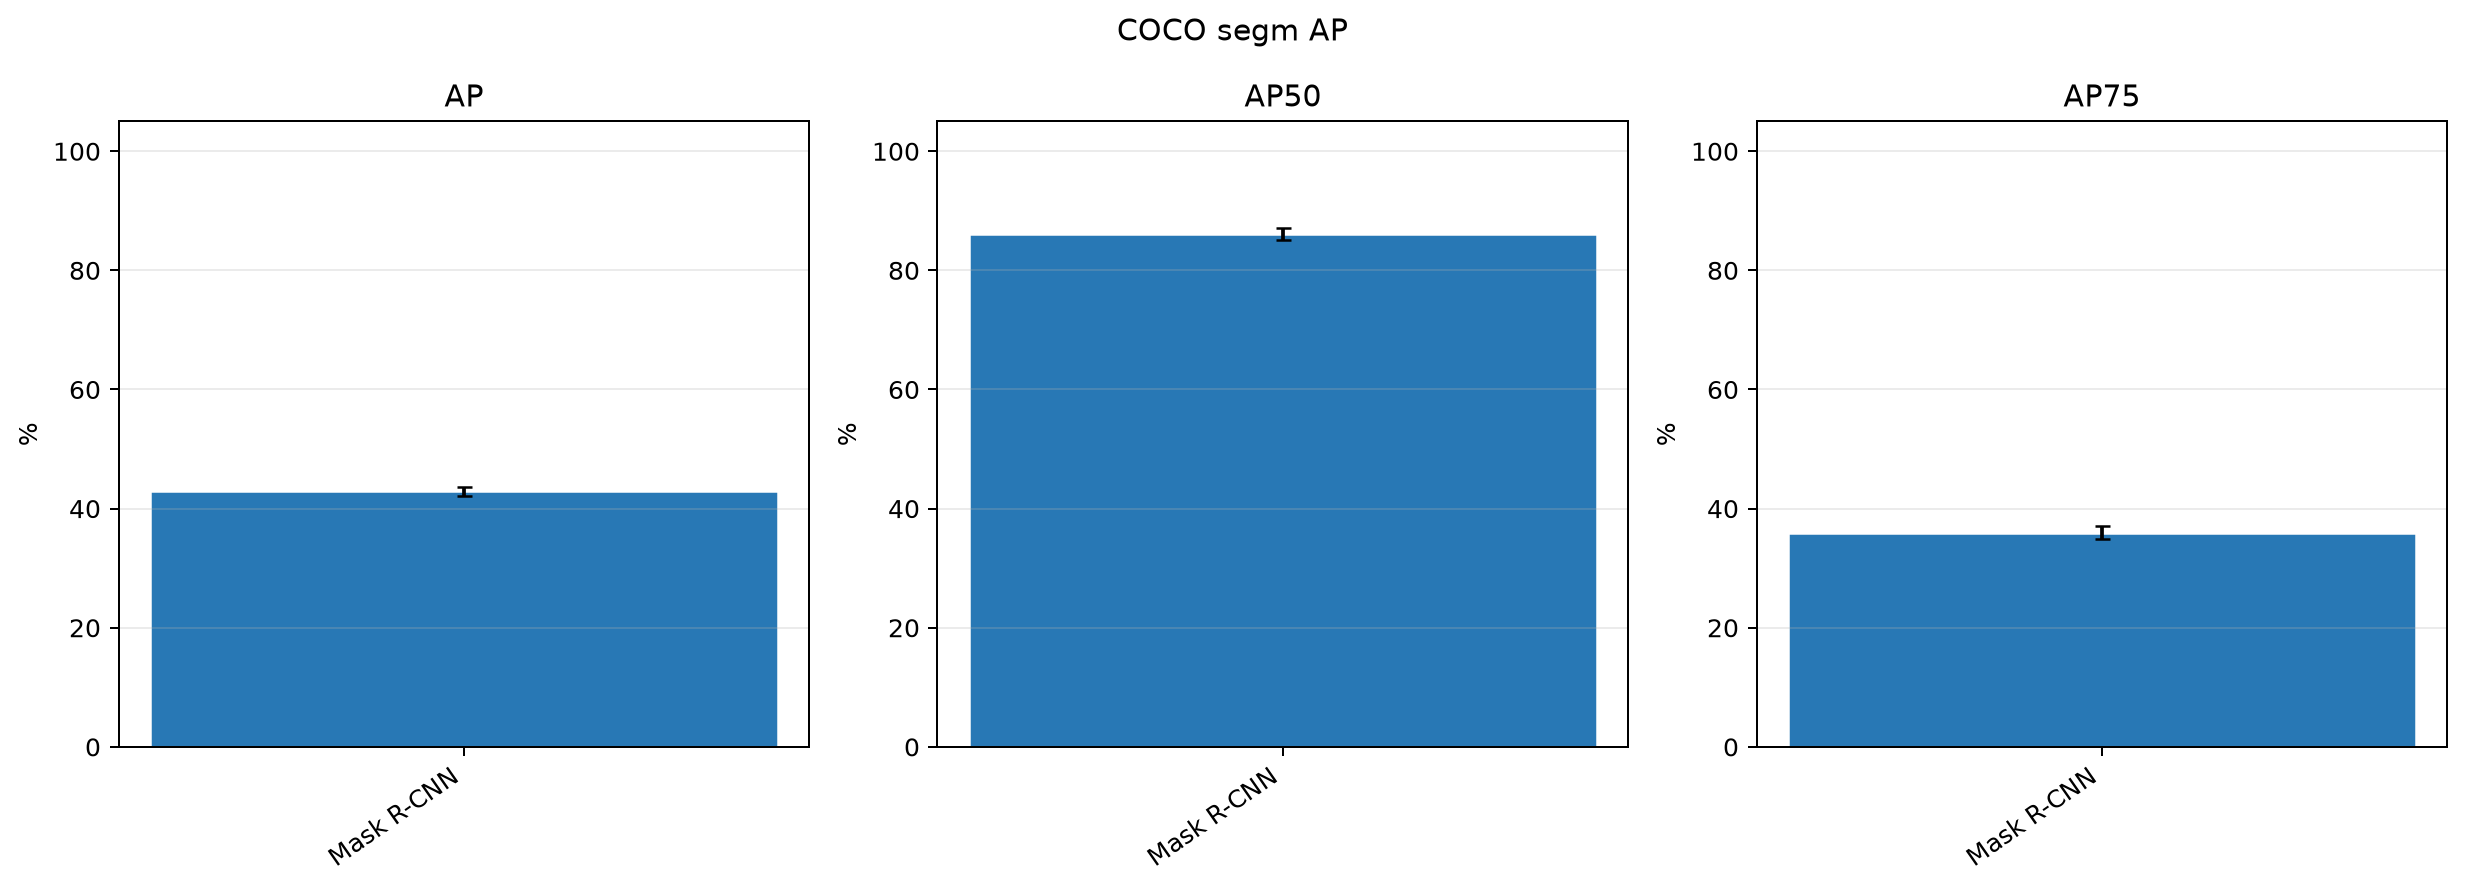
\includegraphics[width=0.8\linewidth]{reports/coco_ap_segm.png}
\caption{AP de segmentação por máscara do Mask R-CNN na rodada atual.}
\label{fig:mask_ap_current}
\end{figure}

% ============================================================
\section{Faster R-CNN}
% ============================================================

Mesma espinha dorsal do Mask R-CNN, sem a etapa de máscara --- apenas detecta a
caixa delimitadora. O objetivo foi isolar a dificuldade de localizar a B-Line da
dificuldade de desenhar sua forma exata. Utiliza o mesmo dataset já registrado, sem
nenhuma conversão adicional.

\begin{table}[H]
\centering
\caption{Faster R-CNN na rodada atual: média $\pm$ desvio-padrão amostral de
três seeds.}
\begin{tabular}{lccc}
\toprule
AP & AP50 & AP75 & P/R/F1 (IoU 0,50) \\
\midrule
$52,37\pm2,38$ & $87,95\pm1,72$ & $55,05\pm4,23$ &
$82,96\pm1,85 / 85,80\pm1,33 / 84,33\pm0,41$ \\
\bottomrule
\end{tabular}
\end{table}

O limiar de confiança que maximiza F1 na validação foi $0,74\pm0,08$. Na execução
anterior havia sido reportado F1 0,85 com limiar 0,53; os números novos usam três
seeds e matching/seleção de threshold padronizados nesta rodada.

\begin{figure}[H]
\centering
\includegraphics[width=0.6\linewidth]{figures/predictions/faster_rcnn_1646467410642.png}
\caption{Exemplo de predição do Faster R-CNN (verde: anotação real; vermelho: caixa
prevista).}
\label{fig:faster_pred}
\end{figure}

\begin{figure}[H]
\centering
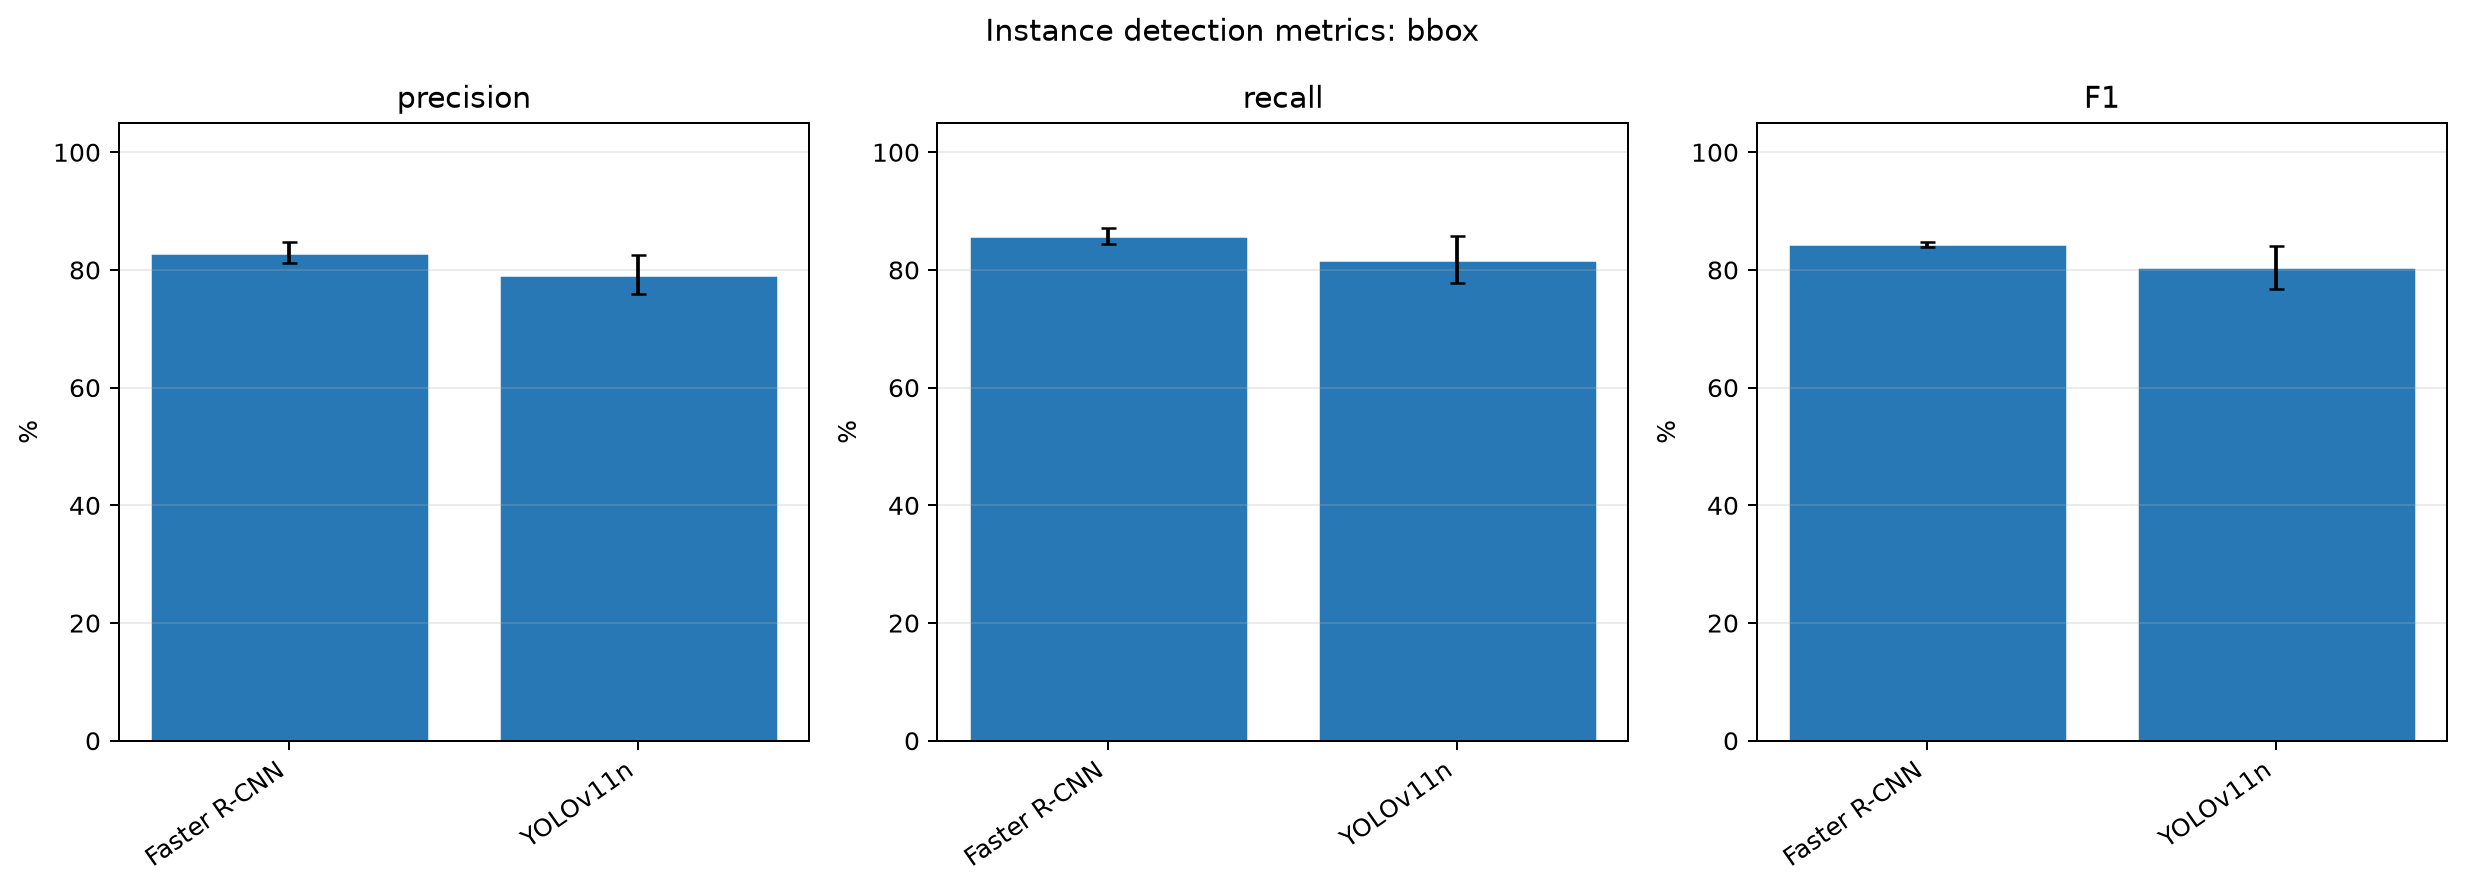
\includegraphics[width=0.8\linewidth]{reports/detection_metrics_bbox.png}
\caption{Precisão, recall e F1 por instância para os detectores de caixa na
rodada atual.}
\label{fig:bbox_metrics}
\end{figure}

% ============================================================
\section{YOLOv11}
% ============================================================

Arquitetura \textit{one-stage}, de família diferente da R-CNN (Ultralytics), usada
para verificar se a dificuldade observada era específica dos modelos R-CNN.
Utilizou-se o \texttt{yolo11n} (variante nano), com o dataset convertido de
polígono para caixa a partir da mesma anotação original, treinado por 31 épocas ---
equivalente ao número de imagens vistas pelo protocolo dos R-CNN (2000 iterações
$\times$ 4 de batch / 256 imagens). Os hiperparâmetros de treino seguiram os padrões
do Ultralytics; não foram forçados os mesmos valores do Detectron2, pois transportar
hiperparâmetros de um framework para outro tende a prejudicar a convergência.

As predições foram exportadas para o formato COCO e avaliadas com o mesmo código
\texttt{pycocotools} utilizado nos demais modelos, não com a métrica nativa do
Ultralytics, para preservar a comparação justa.

\begin{table}[H]
\centering
\caption{YOLOv11n na rodada atual: média $\pm$ desvio-padrão amostral de três
seeds.}
\begin{tabular}{lccc}
\toprule
AP & AP50 & AP75 & P/R/F1 (IoU 0,50) \\
\midrule
$55,86\pm0,99$ & $85,26\pm2,14$ & $59,39\pm2,66$ &
$79,20\pm3,32 / 81,74\pm3,98 / 80,45\pm3,63$ \\
\bottomrule
\end{tabular}
\end{table}

O limiar de confiança médio escolhido na validação foi $0,38\pm0,04$. A execução
anterior reportava F1 0,82 com limiar 0,53; esse valor foi substituído pela
avaliação de três seeds mostrada acima.

\begin{figure}[H]
\centering
\includegraphics[width=0.6\linewidth]{figures/predictions/yolo_1646467410642.png}
\caption{Exemplo de predição do YOLOv11 (verde: anotação real; vermelho: caixa
prevista).}
\label{fig:yolo_pred}
\end{figure}

% ============================================================
\section{Comparação entre os Três Modelos de Caixa}
% ============================================================

\begin{table}[H]
\centering
\caption{Comparação atual de AP de caixa entre Mask R-CNN, Faster R-CNN e
YOLOv11n (média $\pm$ desvio-padrão de três seeds).}
\begin{tabular}{lccc}
\toprule
Modelo & AP & AP50 & AP75 \\
\midrule
Mask R-CNN (caixa) & $56,12\pm1,74$ & $91,23\pm2,01$ & $59,89\pm4,13$ \\
Faster R-CNN & $52,37\pm2,38$ & $87,95\pm1,72$ & $55,05\pm4,23$ \\
YOLOv11n & $55,86\pm0,99$ & $85,26\pm2,14$ & $59,39\pm2,66$ \\
\bottomrule
\end{tabular}
\end{table}

Na rodada atual, o AP de caixa varia de $52,37\%$ (Faster R-CNN) a $56,12\%$
(Mask R-CNN); YOLOv11n obteve $55,86\%$. A diferença entre as médias é descritiva,
e a variação entre seeds deve ser considerada. As arquiteturas usam protocolos de
treino parcialmente diferentes.

\begin{figure}[H]
\centering
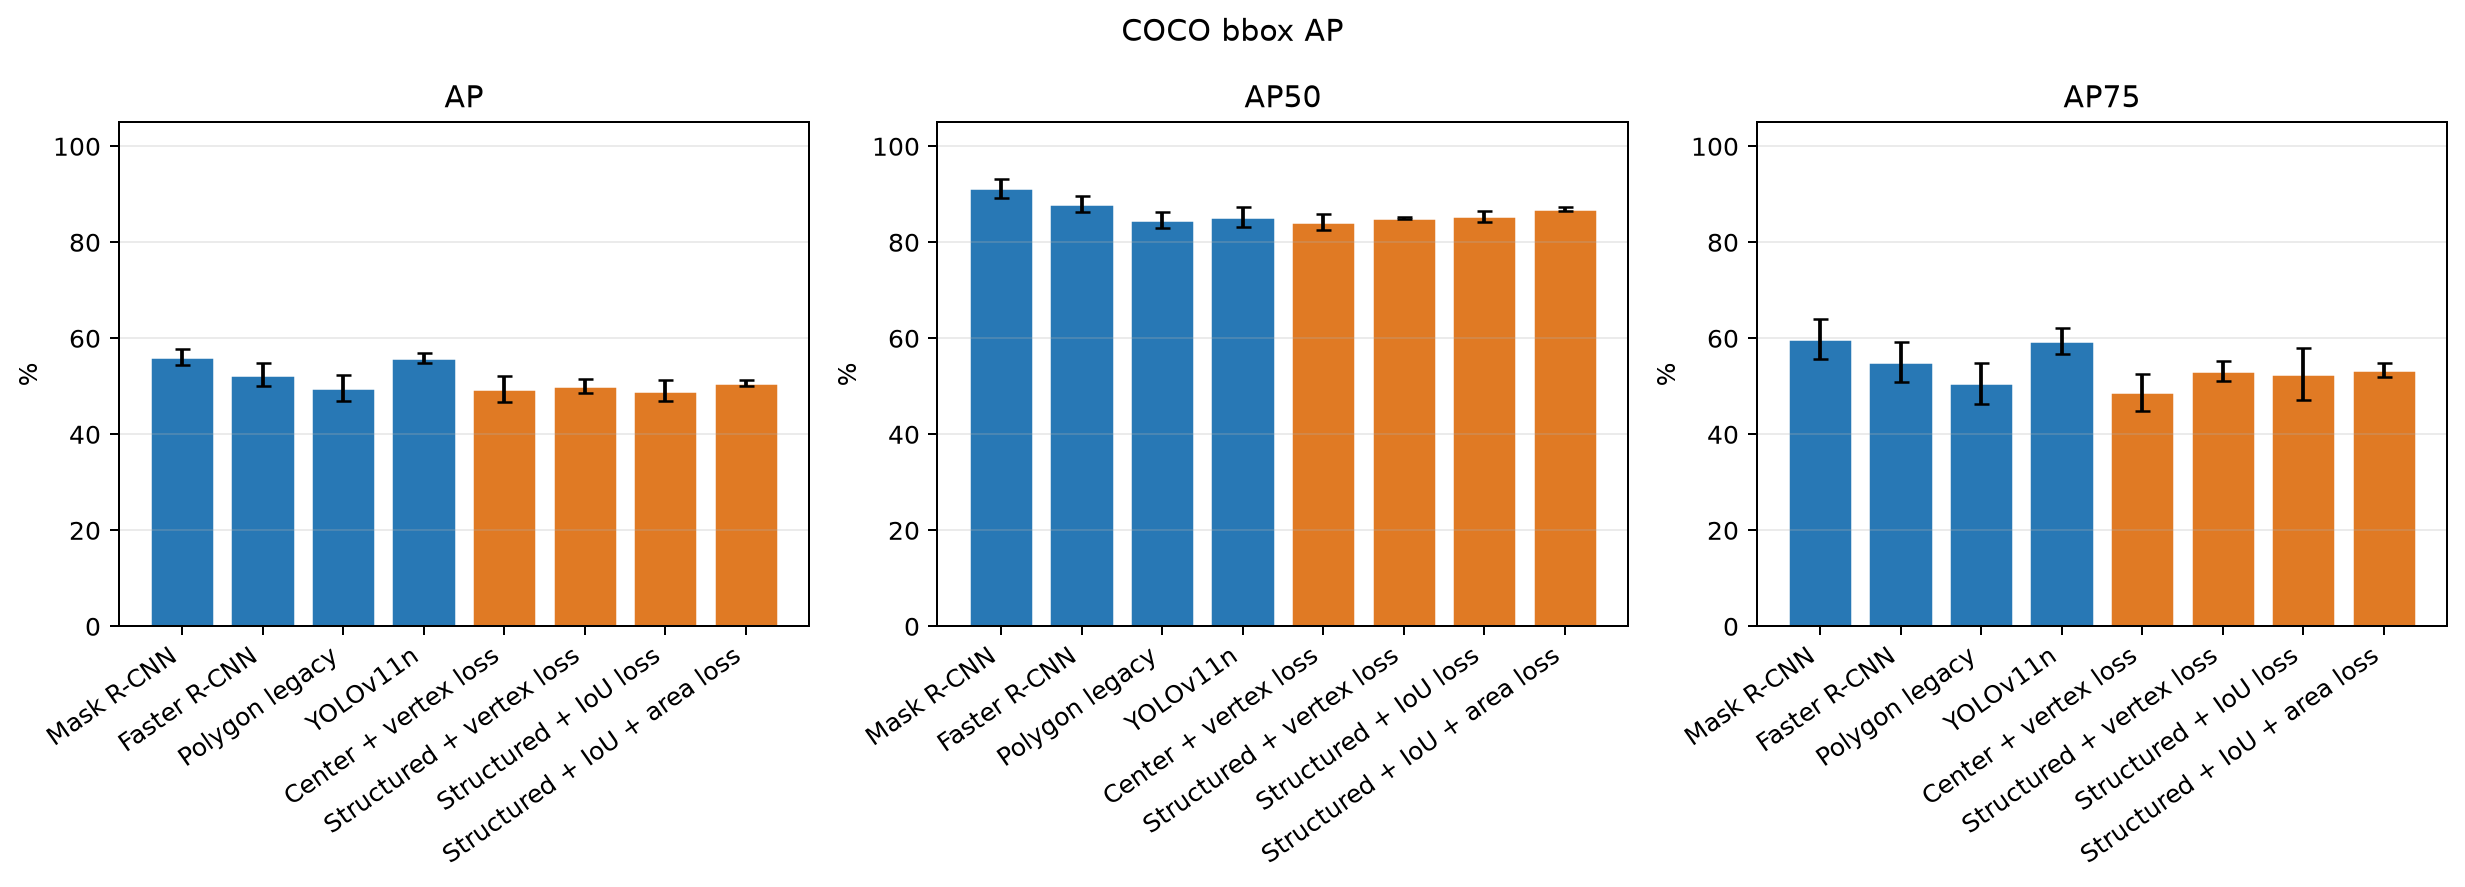
\includegraphics[width=0.7\linewidth]{reports/coco_ap_bbox.png}
\caption{Comparação atual de AP/AP50/AP75 para os detectores de caixa.}
\label{fig:comparison}
\end{figure}

% ============================================================
\section{Polygon Head --- Primeira Tentativa (Heatmap)}
% ============================================================

Em vez de uma máscara livre, a proposta da Polygon Head é prever diretamente os 4
vértices do quadrilátero. Na primeira tentativa, reaproveitou-se a infraestrutura
de Keypoint R-CNN já disponível no Detectron2 (originalmente concebida para pose
humana, com 17 pontos), adaptada para 4 pontos --- cada vértice tratado como um
ponto-chave localizado por um mapa de calor espacial. A opção por reaproveitar essa
infraestrutura, em vez de implementar algo do zero, teve como objetivo evitar
reimplementar, sem GPU disponível para testes interativos, as partes mais
arriscadas: a transformação correta dos pontos quando a imagem sofre corte ou
espelhamento durante o treino.

\begin{table}[H]
\centering
\caption{Resultados exploratórios de execução única da Polygon Head heatmap,
preservados como registro das primeiras tentativas.}
\begin{tabular}{lccccc}
\toprule
Configuração & AP & AP50 & AP75 & Melhor F1 & \% polígono inválido \\
\midrule
Resolução padrão & 15,0 & 37,1 & 11,9 & 0,49 & 6,7\% \\
Resolução dobrada & 3,8 & 10,8 & 2,7 & 0,25 & 20,4\% \\
\bottomrule
\end{tabular}
\end{table}

\noindent \textit{Polígono inválido}: os 4 vértices, conectados na ordem prevista,
formam uma figura que se autointersecciona --- não é um quadrilátero simples.

Aumentar a resolução do mapa de calor piorou o resultado em vez de melhorá-lo. Com
poucos dados (256 imagens) e poucas iterações, um alvo de classificação mais fino
é mais difícil de aprender, não mais fácil. Além disso, o heatmap trata os 4
vértices como classificações independentes entre si --- nada na arquitetura obriga
os pontos a formarem uma figura geometricamente coerente, o que explica a taxa de
autointersecção observada.

Para permitir comparação pelo mesmo avaliador, o polígono previsto foi convertido
em uma região preenchida e avaliado pelo COCOeval de segmentação, com a métrica
denominada \texttt{segm\_polygon}. O avaliador é comum, mas a saída geométrica não
é idêntica à máscara livre do Mask R-CNN; essa distinção é mantida nas
interpretações.

% ============================================================
\section{Polygon Head --- Regressão Direta de Vértice}
% ============================================================

Diante do diagnóstico de que o problema estava no paradigma de classificação por
mapa de calor, a alternativa foi prever diretamente as coordenadas $(x, y)$ de cada
vértice --- regressão contínua em vez de classificação em grade. Como essa opção
não existe pronta no Detectron2, foi implementada uma cabeça de rede nova: quatro
camadas convolucionais, um \textit{pooling} global e duas camadas densas,
terminando em 8 números (4 vértices $\times$ 2 coordenadas) por objeto detectado. A
função de perda é \textit{smooth-L1}, comparando a posição prevista com a real,
ambas normalizadas em relação à própria caixa do objeto --- a mesma técnica já
utilizada pela regressão de \textit{bounding box} do Detectron2.

\begin{table}[H]
\centering
\caption{Resultados exploratórios de execução única da regressão direta, mantidos
como registro das primeiras tentativas.}
\begin{tabular}{lccccc}
\toprule
Configuração & AP & AP50 & AP75 & Melhor F1 & Recall@0,5 \\
\midrule
Sem restrição na saída (melhor) & 12,2 & 54,2 & 1,4 & 0,63 & 0,74 \\
Com sigmoid na saída & 4,3 & 22,9 & 0,1 & 0,37 & 0,42 \\
Com penalidade suave de escape & 8,2 & 35,3 & 0,1 & 0,46 & 0,55 \\
\bottomrule
\end{tabular}
\end{table}

Nas três variantes, a taxa de polígono autointersectado caiu para 0\% (contra
6,7--20,4\% do heatmap) --- a regressão direta resolve por completo esse problema
estrutural.

A versão sem restrição, apesar de superior às demais, produzia polígonos cerca de
20\% maiores que o real, e 88\% das predições apresentavam algum vértice fora da
própria caixa prevista, já que nada na arquitetura impedia isso. Duas correções
foram testadas. A primeira, uma função sigmoide forçando a saída entre 0 e 1,
piorou o resultado: os alvos reais concentram-se exatamente nos valores extremos
(0 e 1, pois a caixa é definida pelos próprios vértices), e é justamente nesse
ponto que o gradiente da sigmoide é menor --- o efeito foi travar o aprendizado em
vez de apenas limitar a saída. A segunda, uma penalidade suave que atua somente
quando o vértice ultrapassa o intervalo válido, também piorou o resultado, e de
forma reveladora: a taxa de vértices fora da caixa não se alterou (permaneceu em
torno de 88\%), evidenciando que esse comportamento nunca foi a causa do problema,
apenas um sintoma correlacionado.

Uma análise exploratória anterior sugeriu caixas previstas 12--16\% maiores que as
anotadas. Esse valor ainda não foi confirmado quantitativamente nas predições da
rodada atual nem pode ser atribuído a todos os detectores. Como os vértices são
parametrizados em relação à proposta, um viés na caixa pode propagar-se para a
geometria; a rotina de análise de viés foi implementada e deve ser executada antes
de tratar essa hipótese como causa estabelecida.

\begin{figure}[H]
\centering
\includegraphics[width=0.6\linewidth]{figures/predictions/polygon_head_1646467410642.png}
\caption{Exemplo de predição da Polygon Head, regressão direta (verde: anotação
real; vermelho: polígono previsto).}
\label{fig:polygon_pred}
\end{figure}

% ============================================================
\section{Polygon Head --- Representação Estruturada e Losses Geométricas}
\label{sec:polygon_ablation}
% ============================================================

Depois das tentativas iniciais com heatmaps e regressão direta, foi implementada
uma nova rodada controlada de ablações. O objetivo foi testar parametrizações e
supervisões geométricas específicas para B-lines, mantendo o dataset, as propostas
e o protocolo Detectron2. Cada configuração foi executada com três seeds.

A configuração \textit{center-relative} representa os quatro vértices como offsets
ao centro da proposta. A configuração \textit{structured} prediz sete parâmetros:
offsets do centro, orientação pela representação periódica
$(\cos 2\theta,\sin 2\theta)$, comprimento e largura em cada extremidade. A
geometria é então reconstruída como quadrilátero. Isso impõe uma estrutura comum
entre os vértices, em contraste com a regressão de oito coordenadas independentes.

Foram comparadas quatro variantes novas: centro relativo com vertex loss;
geometria estruturada com vertex loss; geometria estruturada com vertex loss mais
IoU poligonal suave; e a última configuração acrescida de loss relativa de área.
A variante legacy com vertex loss também foi reexecutada como referência nas
baselines. A loss de IoU é uma aproximação diferenciável obtida por rasterização
suave em grade fixa $32\times32$; ela orienta o treinamento, enquanto COCOeval
continua sendo a métrica de avaliação.

Na rodada atual, a geometria estruturada com vertex loss elevou o AP poligonal
médio de $14,36\%$ (legacy) para $18,57\%$. Adicionar somente IoU suave resultou
em AP médio de $17,82\%$, mas o AP75 subiu de $2,08\%$ para $5,87\%$. A
configuração com IoU e área alcançou o maior AP poligonal ($20,15\%$), AP50
($60,08\%$) e F1 por instância ($65,83\%$). O AP75 permaneceu baixo
($5,26\%$), indicando que a localização precisa ainda é difícil. As diferenças
são descritivas; três seeds e 75 imagens não bastam para afirmar significância
estatística.

A tabela~\ref{tab:resumo_comparativo} reúne os resultados antigos preservados e
os valores atuais. Os valores das primeiras tentativas permanecem identificados
como execução única; eles não foram reexecutados na nova matriz e seus limiares e
protocolos podem diferir dos atuais.

\begin{figure}[H]
\centering
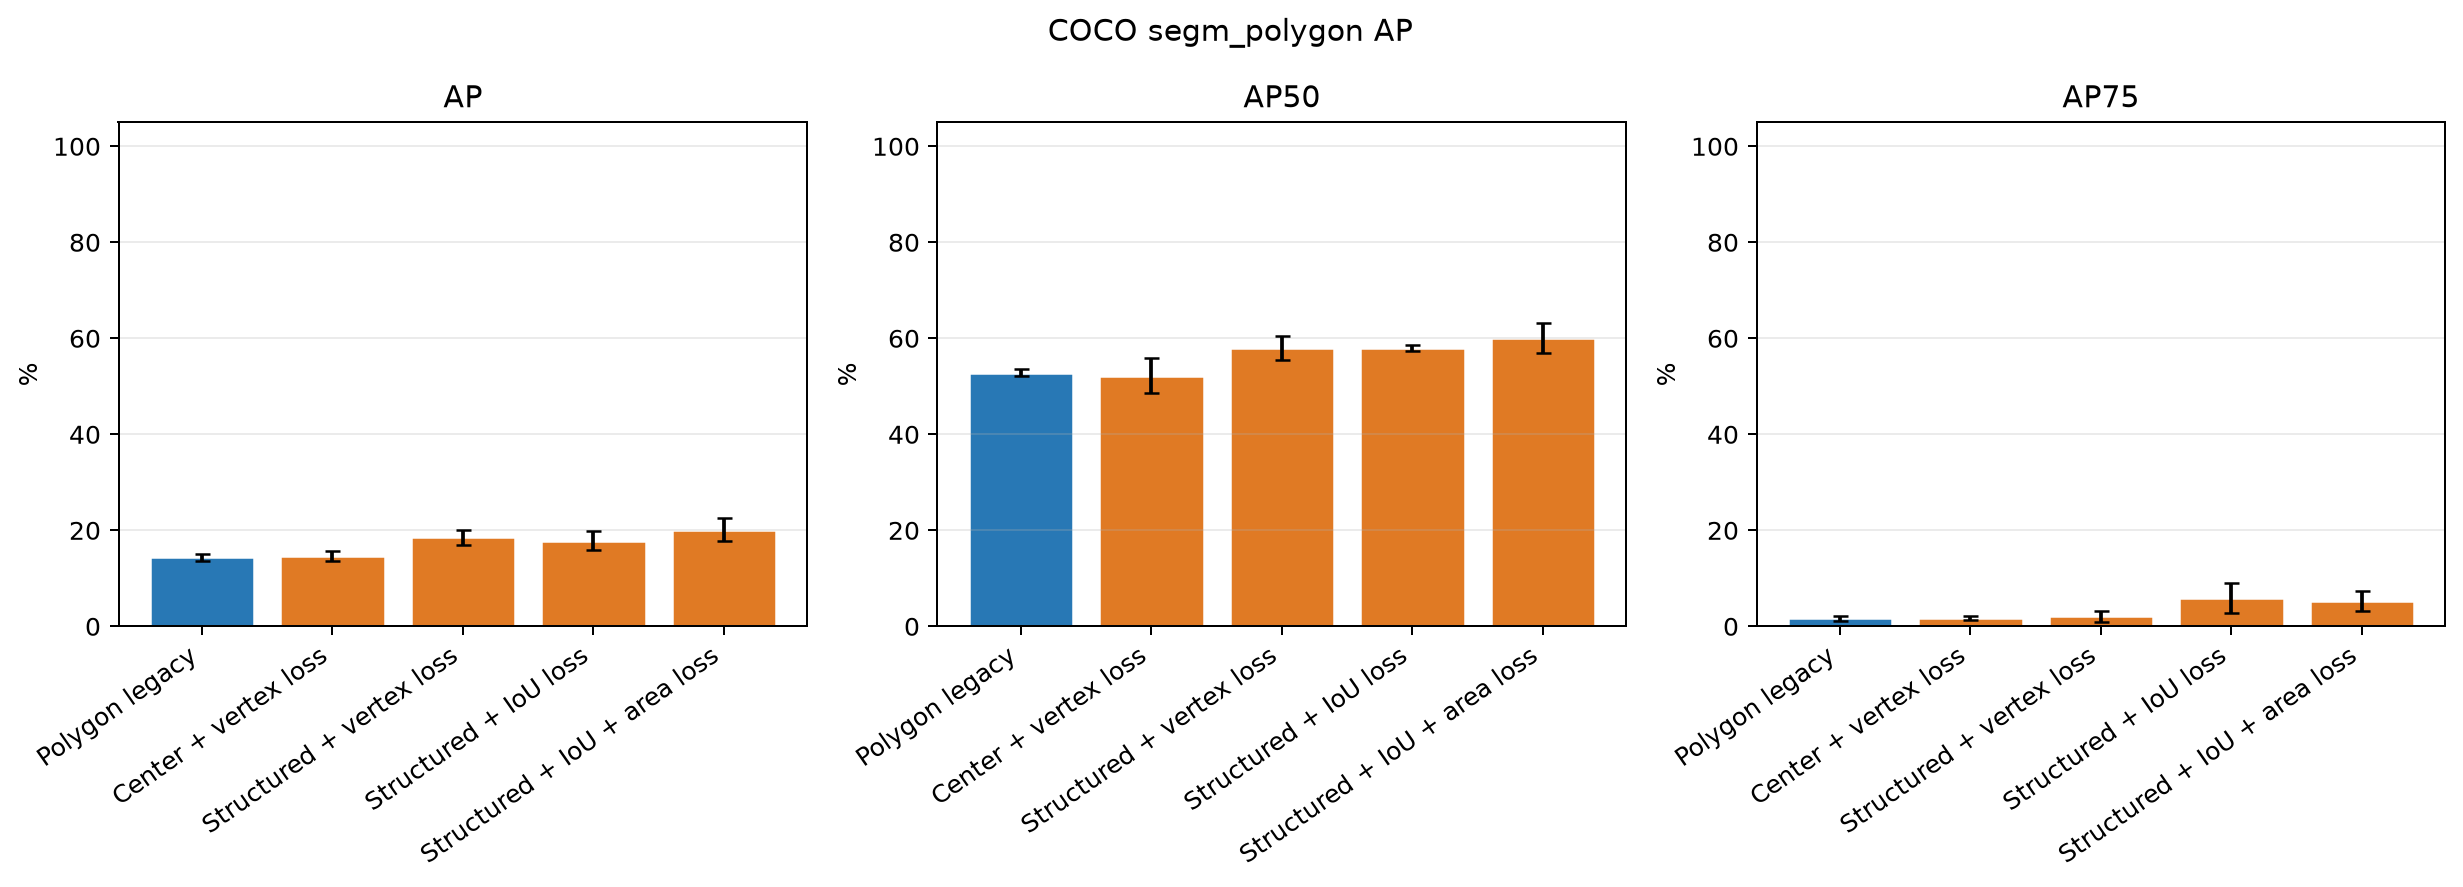
\includegraphics[width=0.8\linewidth]{reports/coco_ap_segm_polygon.png}
\caption{AP, AP50 e AP75 para as variantes poligonais atuais, agregadas em três
seeds.}
\label{fig:polygon_ablation_ap}
\end{figure}

\begin{figure}[H]
\centering
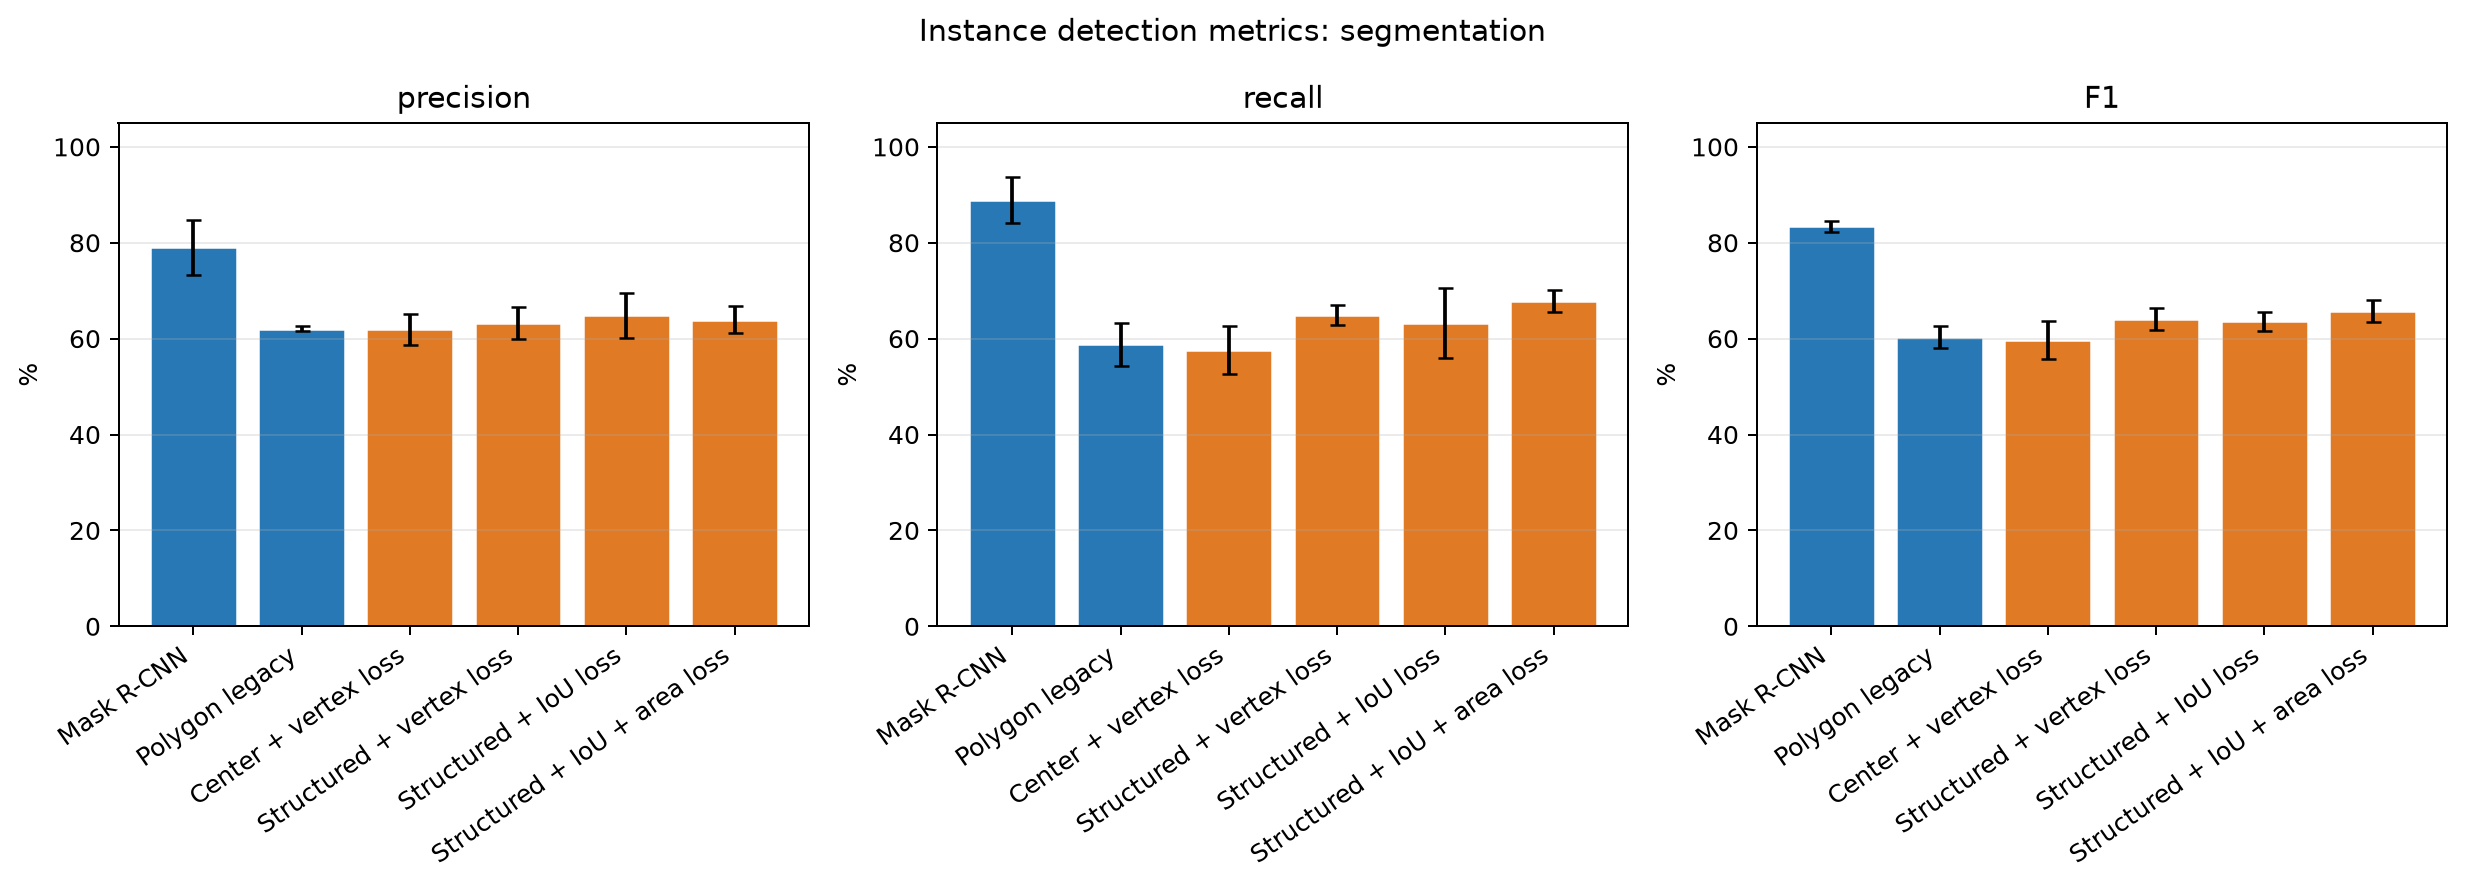
\includegraphics[width=0.8\linewidth]{reports/detection_metrics_segmentation.png}
\caption{Precisão, recall e F1 por instância para as saídas de máscara e
poligonais atuais. O limiar é escolhido na validação.}
\label{fig:polygon_ablation_prf1}
\end{figure}

\begin{figure}[H]
\centering
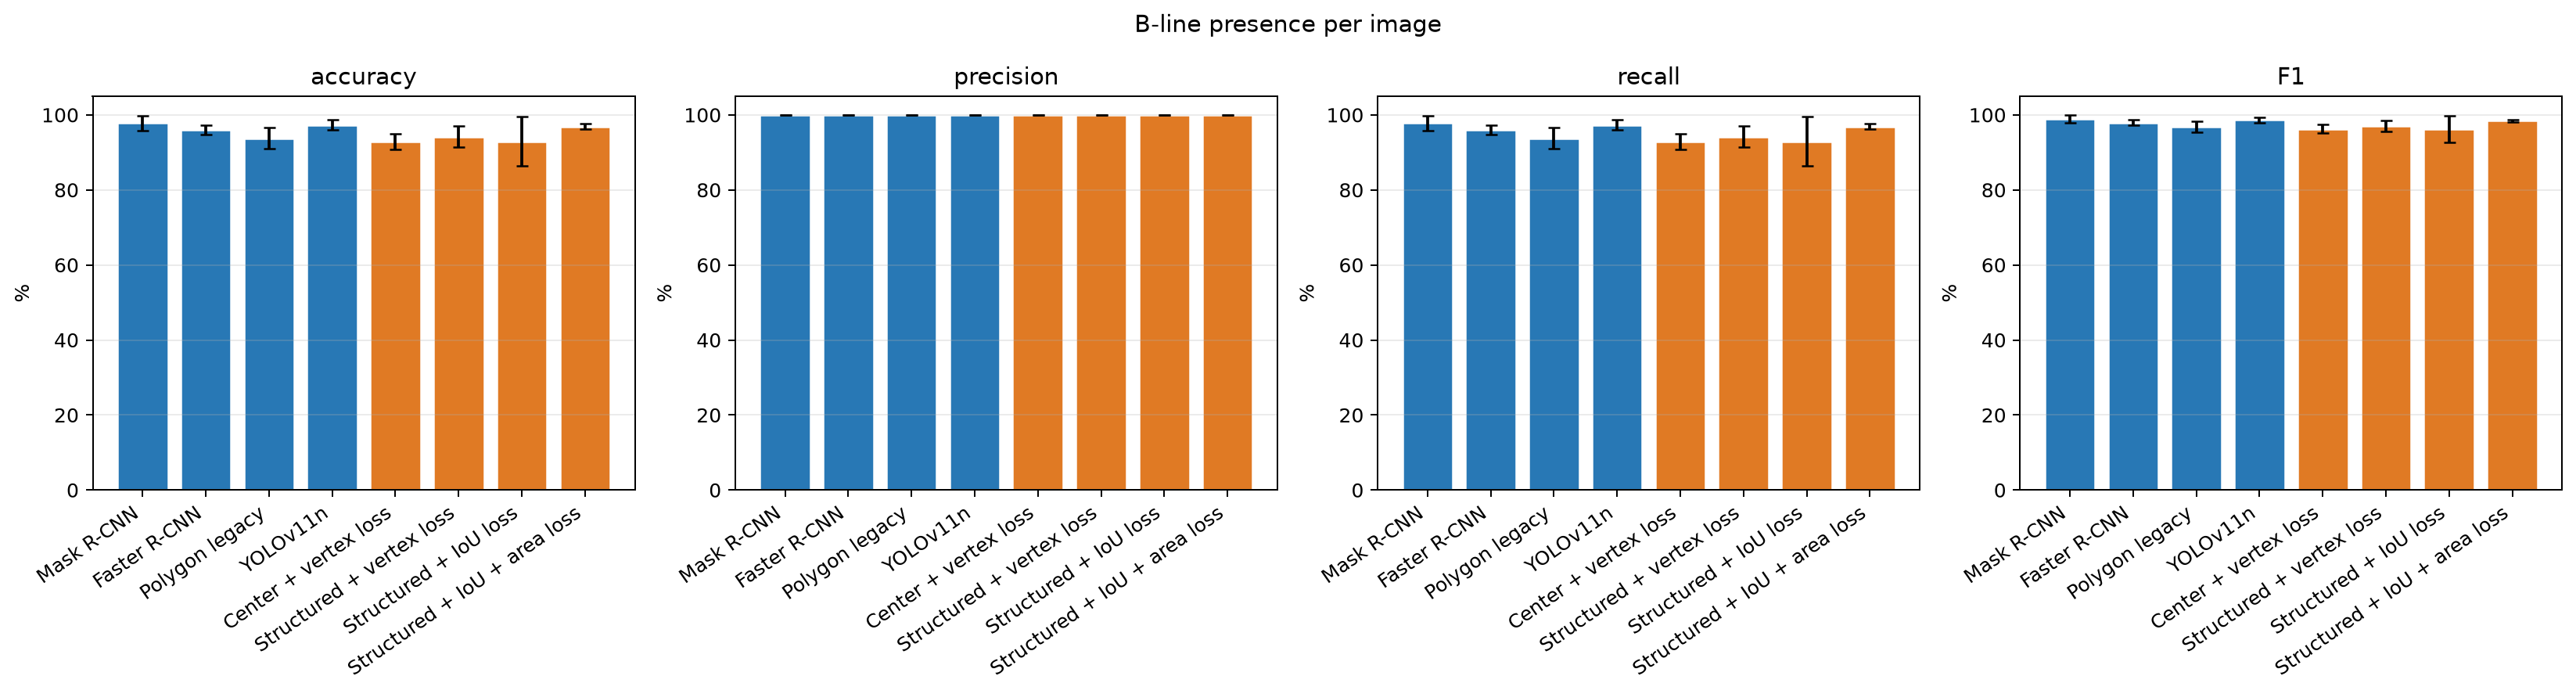
\includegraphics[width=0.8\linewidth]{reports/image_presence_metrics.png}
\caption{Métricas de presença por imagem para a rodada atual. Como não há imagens
negativas no split de validação, a figura não permite medir especificidade.}
\label{fig:image_presence}
\end{figure}

% ============================================================
\section{Resumo Geral}
\label{sec:resumo}
% ============================================================

\small
\setlength{\tabcolsep}{2pt}
\renewcommand{\arraystretch}{1.12}
\begin{longtable}{@{}p{3.5cm}p{4.3cm}p{4.8cm}p{2.5cm}@{}}
\caption{Comparação consolidada dos resultados anteriores preservados e da rodada
atual. Os valores estão em porcentagem; os atuais são média $\pm$ desvio-padrão amostral de três seeds;
os resultados das primeiras tentativas são execuções únicas.}
\label{tab:resumo_comparativo}\\
\toprule
Modelo / configuração & AP / AP50 / AP75 & Precisão / recall / F1 por instância &
Presença: acurácia / F1 \\
\midrule
\endfirsthead
\multicolumn{4}{c}{\tablename\ \thetable{} --- continuação}\\
\toprule
Modelo / configuração & AP / AP50 / AP75 & Precisão / recall / F1 por instância &
Presença: acurácia / F1 \\
\midrule
\endhead
\midrule
\multicolumn{4}{r}{Continua na próxima página}\\
\endfoot
\bottomrule
\endlastfoot
Mask R-CNN, máscara (atual) & $42,88\pm0,70\allowbreak / 86,14\pm0,98\allowbreak / 35,98\pm1,09$ & $79,01\pm5,83\allowbreak / 88,99\pm4,79\allowbreak / 83,47\pm1,15$ & $97,78\pm2,04\allowbreak / 98,87\pm1,04$ \\
Mask R-CNN, caixa (atual) & $56,12\pm1,74\allowbreak / 91,23\pm2,01\allowbreak / 59,89\pm4,13$ & -- & -- \\
Faster R-CNN, caixa (atual) & $52,37\pm2,38\allowbreak / 87,95\pm1,72\allowbreak / 55,05\pm4,23$ & $82,96\pm1,85\allowbreak / 85,80\pm1,33\allowbreak / 84,33\pm0,41$ & $96,00\pm1,33\allowbreak / 97,96\pm0,69$ \\
YOLOv11n, caixa (atual) & $55,86\pm0,99\allowbreak / 85,26\pm2,14\allowbreak / 59,39\pm2,66$ & $79,20\pm3,32\allowbreak / 81,74\pm3,98\allowbreak / 80,45\pm3,63$ & $97,33\pm1,33\allowbreak / 98,65\pm0,68$ \\
Polygon heatmap, resolução padrão (inicial) & $15,0 / 37,1 / 11,9$ & $-- / -- / 49$ & -- \\
Polygon heatmap, resolução dobrada (inicial) & $3,8 / 10,8 / 2,7$ & $-- / -- / 25$ & -- \\
Polygon regressão com sigmoid (inicial) & $4,3 / 22,9 / 0,1$ & $-- / 42 / 37$ & -- \\
Polygon regressão com penalidade (inicial) & $8,2 / 35,3 / 0,1$ & $-- / 55 / 46$ & -- \\
Polygon legacy, vertex loss (atual) & $14,36\pm0,73\allowbreak / 52,86\pm0,70\allowbreak / 1,63\pm0,44$ & $62,09\pm0,60\allowbreak / 58,84\pm4,46\allowbreak / 60,36\pm2,35$ & $93,78\pm2,78\allowbreak / 96,77\pm1,49$ \\
Polygon center-relative, vertex loss (atual) & $14,63\pm1,01\allowbreak / 52,16\pm3,65\allowbreak / 1,66\pm0,43$ & $61,98\pm3,26\allowbreak / 57,68\pm5,02\allowbreak / 59,71\pm3,89$ & $92,89\pm2,04\allowbreak / 96,31\pm1,10$ \\
Polygon structured, vertex loss (atual) & $18,57\pm1,54\allowbreak / 57,98\pm2,43\allowbreak / 2,08\pm1,09$ & $63,19\pm3,37\allowbreak / 64,93\pm2,19\allowbreak / 64,02\pm2,30$ & $94,22\pm2,78\allowbreak / 97,01\pm1,46$ \\
Polygon structured, IoU suave (atual) & $17,82\pm2,01\allowbreak / 57,92\pm0,58\allowbreak / 5,87\pm3,10$ & $64,86\pm4,65\allowbreak / 63,19\pm7,29\allowbreak / 63,64\pm1,96$ & $92,89\pm6,58\allowbreak / 96,23\pm3,61$ \\
Polygon structured, IoU + área (atual) & $20,15\pm2,44\allowbreak / 60,08\pm3,10\allowbreak / 5,26\pm2,11$ & $63,98\pm2,82\allowbreak / 67,83\pm2,30\allowbreak / 65,83\pm2,32$ & $96,89\pm0,77\allowbreak / 98,42\pm0,40$ \\
\end{longtable}

\normalsize
{\footnotesize
Em cada trio, a ordem é AP/AP50/AP75 ou precisão/recall/F1, conforme o cabeçalho.
Os AP atuais são de caixa para os detectores bbox, de máscara para Mask R-CNN
(máscara) e de região poligonal preenchida (\texttt{segm\_polygon}) para Polygon
Head; a avaliação usa COCOeval, mas as saídas máscara e polígono não são a mesma
representação. P/R/F1 atuais usam IoU 0,50 e limiar escolhido na validação. Nas
linhas iniciais, F1 e recall são os valores do relatório exploratório anterior, sem
recalcular precisão quando ela não foi reportada. A presença por imagem só foi
consolidada para a rodada atual. Como as 75 imagens de validação são positivas,
acurácia de presença coincide com recall e não mede especificidade.\par}

Os resultados atuais mostram que o AP de caixa dos baselines varia entre
$52,37\%$ e $56,12\%$. Para a Polygon Head, a representação estruturada com IoU e
área tem o maior AP médio atual ($20,15\%$) e F1 por instância ($65,83\%$), mas o
AP75 permanece baixo. A melhoria em relação à variante legacy é promissora, mas
descritiva: não demonstra significância estatística e não estabelece superioridade
em teste independente. O Mask R-CNN obtém AP de máscara $42,88\%$; como máscara
livre e polígono têm saídas distintas, essa diferença deve ser interpretada como
referência, não como comparação perfeitamente equivalente.

% ============================================================
\section{Limitações e Trabalhos Futuros}
\label{sec:limitacoes}
% ============================================================

\begin{itemize}
\item Os resultados da nova rodada usam três seeds por configuração e informam
média e desvio-padrão amostral. Ainda não foram calculados intervalos de confiança
pareados por imagem; as diferenças entre médias não demonstram, por si só,
significância estatística.

\item Na nova rodada, a seleção do checkpoint é alinhada à tarefa: bbox/AP para
Faster R-CNN, segm/AP para Mask R-CNN e segm\_polygon/AP para Polygon Head. Os
resultados exploratórios antigos de Polygon Head não têm logs completos para
confirmar a seleção de checkpoint usada naquela época.

\item O \textit{flip} horizontal foi desativado nas rodadas poligonais atuais.
O código agora oferece flip com reordenação canônica dos vértices, mas essa
variante não foi treinada. Mask R-CNN, Faster R-CNN e YOLO usam augmentations
próprias de seus pipelines; portanto, as famílias não compartilham um protocolo
de augmentations perfeitamente idêntico.

\item A métrica \texttt{segm\_polygon} não corresponde a uma AP de máscara por
pixel no sentido literal --- é o polígono avaliado pelo mesmo COCOeval de
segmentação, uma comparação justa, mas que deve ser identificada como tal.

\item Não existe, até o momento, um conjunto de teste anotado separado do de
validação.

\item A hipótese de caixas 12--16\% maiores veio de uma análise exploratória
anterior. A rotina de viés de bbox existe, mas ainda não foi executada nas
predições atuais; não se deve atribuir esse efeito a todos os detectores sem essa
medição.

\item Foram implementadas métricas geométricas (erro de vértices, IoU e área
poligonais, orientação, dimensões e taxa de polígonos inválidos) e categorias de
erro, mas os resultados não foram incluídos na agregação atual. O bootstrap
pareado por imagem também existe no código e ainda precisa ser executado. Essas
análises podem ser feitas a partir das predições salvas, sem repetir os treinos;
os comandos estão em \texttt{docs/REMOTE\_RUNBOOK.md}.

\item As métricas thresholdizadas e de presença são calculadas na validação. O
limiar de confiança foi escolhido para maximizar F1 nesse mesmo split. Além disso,
como todas as imagens de validação são positivas, métricas de presença não medem
especificidade nem desempenho em exames sem B-lines.

\item A loss de IoU suave é uma aproximação rasterizada de treinamento, não uma
loss analítica exata de interseção entre polígonos. Uma loss dedicada de fronteira
e a tarefa auxiliar de origem pleural não foram implementadas. As anotações atuais
não incluem pontos de origem pleural, então essa hipótese requer rótulos próprios.

\item \textbf{Lacuna de revisão de literatura.} O desenho da Polygon Head e de sua
função de perda foi realizado por engenharia própria --- reaproveitando o padrão
de regressão de caixa do Detectron2 e por diagnóstico dos próprios experimentos
--- sem revisão prévia da literatura específica sobre detecção de quadriláteros e
objetos orientados. Trabalhos diretamente relevantes ainda não consultados
incluem: EAST e TextBoxes++ (detecção de texto via 4 cantos, com supervisão densa
por pixel, não um único vetor por objeto); Gliding Vertex e RoI Transformer
(parametrizam o vértice como deslocamento a partir de uma caixa alinhada, uma
regressão mais restrita do que a utilizada neste trabalho); e CornerNet (heatmap
de cantos com mecanismo adicional para garantir coerência entre os pontos,
ausente na variante heatmap aqui implementada). Essa lacuna deve orientar a
próxima rodada de experimentos.
\end{itemize}

\end{document}
